\documentclass{article}

\usepackage[english]{babel}
\usepackage[letterpaper,top=2cm,bottom=2cm,left=3cm,right=3cm,marginparwidth=1.75cm]{geometry}
\setlength{\parindent}{0pt}

\usepackage{amsmath}
\usepackage{amsthm}
\usepackage{amssymb}
\usepackage{graphicx}
\usepackage{float}
\usepackage{listings}
\usepackage[colorlinks=true, allcolors=blue]{hyperref}
\usepackage{xcolor}

\lstset{
  basicstyle=\ttfamily\small,
  numbers=left,
  numberstyle=\tiny,
  stepnumber=1,
  numbersep=8pt,
  backgroundcolor=\color{gray!10},
  frame=single,
  rulecolor=\color{gray!60},
  tabsize=2,
  captionpos=b,
  breaklines=true,
  breakatwhitespace=true,
  showstringspaces=false,
  keywordstyle=\color{blue},
  commentstyle=\color{green!50!black},
  stringstyle=\color{orange},
}

\DeclareMathOperator{\sign}{sign}
\DeclareMathOperator{\supp}{supp}
\DeclareMathOperator{\VC}{VCdim}

\newcommand{\EE}{\mathbb{E}}
\newcommand{\PP}{\mathbb{P}}
\newcommand{\cB}{\mathcal{B}}
\newcommand{\cD}{\mathcal{D}}
\newcommand{\cH}{\mathcal{H}}
\newcommand{\cI}{\mathcal{I}}
\newcommand{\one}{\mathbf{1}}

\title{DSC 291: Learning Theory Assignment 6}
\author{Tongle Shen}

\begin{document}
\maketitle

\section{\texorpdfstring{Part A: Boosting Sparse Linear Predictors and the $\ell_1$ Margin}{Part A: Boosting Sparse Linear Predictors and the l1 Margin}}

\subsection{Problem 1. A Coordinate Weak Learner from Sparse Margin}

Fix any distribution $Q$ supported on examples satisfying
$$
y\langle w^\star,\phi(x)\rangle \ge 1,
\qquad
\|w^\star\|_0 \le s.
$$
Write
$$
\mu_j := \EE_Q[y\,\phi_j(x)].
$$
Taking expectation in the margin inequality gives
$$
1
\le
\EE_Q\!\left[y\sum_{j=1}^d w_j^\star \phi_j(x)\right]
=
\sum_{j=1}^d w_j^\star \mu_j.
$$
Therefore
$$
1
\le
\sum_{j=1}^d |w_j^\star|\,|\mu_j|
\le
\|w^\star\|_1 \max_{j\in[d]} |\mu_j|.
$$
Hence there exists some coordinate $j^\star$ such that
$$
|\mu_{j^\star}|
\ge
\frac{1}{\|w^\star\|_1}.
$$
Now choose
$$
\sigma^\star := \sign(\mu_{j^\star}),
\qquad
b(x) := b_{j^\star,\sigma^\star}(x)=\sigma^\star \phi_{j^\star}(x).
$$
Then
$$
\EE_Q[y\,b(x)]
=
\sigma^\star \EE_Q[y\,\phi_{j^\star}(x)]
=
|\mu_{j^\star}|
\ge
\frac{1}{\|w^\star\|_1}.
$$
Since
$$
\frac12 - L_Q(b) = \frac{\EE_Q[y\,b(x)]}{2},
$$
we obtain
$$
L_Q(b)
\le
\frac12 - \frac{1}{2\|w^\star\|_1}.
$$
Because $w^\star$ is $s$-sparse and $\|w^\star\|_\infty \le B$,
$$
\|w^\star\|_1 \le sB,
$$
so also
$$
L_Q(b)
\le
\frac12 - \frac{1}{2sB}.
$$

\subsubsection{\texorpdfstring{Weighted ERM over $\cB$}{Weighted ERM over B}}

Given weighted examples
$$
(x_i,y_i,D_i)_{i=1}^n,
\qquad
D_i \ge 0,
\qquad
\sum_{i=1}^n D_i = 1,
$$
the weighted error of $b_{j,\sigma}$ is
$$
L_D(b_{j,\sigma})
=
\sum_{i=1}^n D_i \one[b_{j,\sigma}(x_i)\ne y_i]
=
\frac12 - \frac12 \sum_{i=1}^n D_i y_i \sigma \phi_j(x_i).
$$
For each coordinate define the weighted correlation
$$
c_j := \sum_{i=1}^n D_i y_i \phi_j(x_i).
$$
For fixed $j$, the better sign is $\sigma=\sign(c_j)$, giving error
$$
\frac12 - \frac{|c_j|}{2}.
$$
So weighted ERM over $\cB$ is:
\begin{itemize}
\item compute all $c_j$ for $j\in[d]$,
\item choose $j^\star\in\arg\max_j |c_j|$,
\item output $b_{j^\star,\sign(c_{j^\star})}$.
\end{itemize}
Computing every $c_j$ requires one pass over the weighted sample and costs $O(nd)$ time.

\subsection{Problem 2. AdaBoost and the Generalization Bound}

Run AdaBoost on the base class $\cB$. By Problem 1, every reweighted distribution encountered by AdaBoost admits a weak learner with error at most
$$
\varepsilon_t \le \frac12 - \gamma,
\qquad
\gamma := \frac{1}{2sB}.
$$
AdaBoost chooses
$$
\alpha_t = \frac12 \log\!\left(\frac{1-\varepsilon_t}{\varepsilon_t}\right),
$$
and its standard normalization factor is
$$
Z_t = 2\sqrt{\varepsilon_t(1-\varepsilon_t)}.
$$
Therefore the empirical training error after $T$ rounds satisfies
$$
\widehat{L}(H_T)
\le
\prod_{t=1}^T Z_t
\le
\left(2\sqrt{\left(\frac12-\gamma\right)\left(\frac12+\gamma\right)}\right)^T
=
\left(\sqrt{1-4\gamma^2}\right)^T.
$$
Using $\sqrt{1-u}\le e^{-u/2}$,
$$
\widehat{L}(H_T)
\le
e^{-2\gamma^2 T}.
$$
Substituting $\gamma=1/(2sB)$ gives
$$
\widehat{L}(H_T)
\le
\exp\!\left(-\frac{T}{2s^2B^2}\right).
$$

To force zero training error on an $n$-point sample, it is enough to make the right-hand side smaller than $1/n$. Thus it suffices to choose
$$
T \ge 2s^2B^2 \log n.
$$

\subsubsection{From Boosting to a Sparse Linear Classifier}

Each weak learner has the form
$$
h_t(x)=\sigma_t \phi_{j_t}(x),
\qquad
\sigma_t \in \{-1,+1\}.
$$
Hence the boosted score can be written as
$$
F_T(x)
=
\sum_{t=1}^T \alpha_t h_t(x)
=
\left\langle
\sum_{t=1}^T \alpha_t \sigma_t e_{j_t},
\phi(x)
\right\rangle.
$$
So the final classifier is
$$
H_T(x)=\sign(F_T(x))=\sign(\langle w_T,\phi(x)\rangle)
$$
for
$$
w_T := \sum_{t=1}^T \alpha_t \sigma_t e_{j_t}.
$$
Its support satisfies
$$
|\supp(w_T)| \le T.
$$

Now apply the sparse-linear VC bound with activated-coordinate budget $T$:
$$
\VC(\cH_T)
=
O\!\left(T\log\!\left(\frac{ed}{T}\right)\right),
$$
where
$$
\cH_T
:=
\left\{
x \mapsto \sign(\langle w,\phi(x)\rangle)
:
\|w\|_0 \le T
\right\}.
$$
Since AdaBoost produces a sample-consistent hypothesis once $T\ge 2s^2B^2\log n$, the realizable VC theorem gives true error at most $\varepsilon$ with probability at least $1-\delta$ provided
$$
n
=
O\!\left(
\frac{
T\log(ed/T)+\log(1/\delta)
}{
\varepsilon
}
\right).
$$
Substituting $T=O(s^2B^2\log n)$ and absorbing the extra logarithms into $\widetilde{O}(\cdot)$ yields
$$
n
=
\widetilde{O}\!\left(
\frac{
s^2B^2\log d+\log(1/\delta)
}{
\varepsilon
}
\right).
$$

\subsubsection{Comparison with Exact Sparse ERM}

Exact sparse ERM has realizable sample complexity
$$
\widetilde{O}\!\left(
\frac{
s\log(ed/s)+\log(1/\delta)
}{
\varepsilon
}
\right),
$$
so boosting pays a statistical price of roughly an extra factor proportional to
$$
\frac{1}{\gamma^2} = s^2B^2.
$$
This is the cost of replacing exact combinatorial search by a weak-learning reduction.

The computational advantage is that each boosting round only needs the $O(nd)$ weighted ERM from Problem 1, so the total training time is
$$
O(ndT)=O(nd\,s^2B^2\log n).
$$
This avoids the hard support-search subproblem of exact sparse ERM.

The parameter $B$ is essential. If the realizing separator has very uneven coefficients, then $\|w^\star\|_1$ can be much larger than $s$, which shrinks the weak edge and increases both the number of rounds and the final generalization complexity.

\subsection{\texorpdfstring{Problem 3. A Hard Construction Showing Why $B$ Matters}{Problem 3. A Hard Construction Showing Why B Matters}}

Let
$$
s=2m+1
\qquad\text{and}\qquad
d=s.
$$
Index the $s$ support points by
$$
0,\ (1,+),\ (1,-),\ \dots,\ (m,+),\ (m,-),
$$
and let every label be $y=+1$.

We construct $s$ coordinates, grouped as one base column, $m$ flip columns, and $m$ carry columns.

\subsubsection{The Feature Matrix}

Let the columns be
$$
c_0,\ f_1,\dots,f_m,\ g_1,\dots,g_m \in \{-1,+1\}^s.
$$
They are defined row-wise as follows.

\textbf{Base column $c_0$.}
$$
c_0(0)=+1,
\qquad
c_0(r,+)=+1,
\qquad
c_0(r,-)=-1.
$$

\textbf{Flip column $f_t$.}
It matches $c_0$ except on the pair $(t,+),(t,-)$, where the signs are flipped:
$$
f_t(0)=+1,
\qquad
f_t(t,+)=-1,
\qquad
f_t(t,-)=+1,
$$
and for $r\ne t$,
$$
f_t(r,+)=+1,
\qquad
f_t(r,-)=-1.
$$

\textbf{Carry column $g_t$.}
Set
$$
g_t(0)=-1.
$$
For a pair indexed by $r$:
\begin{itemize}
\item if $r<t$, then $g_t(r,+)=g_t(r,-)=-1$;
\item if $r=t$, then $g_t(t,+)=g_t(t,-)=+1$;
\item if $r>t$, then $g_t(r,+)=+1$ and $g_t(r,-)=-1$.
\end{itemize}

Let $M\in\{-1,+1\}^{s\times s}$ be the matrix whose columns are
$$
M=[c_0\ f_1\ \cdots\ f_m\ g_1\ \cdots\ g_m].
$$

\subsubsection{Every Coordinate Has Exponentially Small Edge}

Assign weights
$$
q_0=1,
\qquad
q_{r,+}=q_{r,-}=2^{r-1}
\quad\text{for }r\in[m].
$$
Let
$$
Z := q_0+\sum_{r=1}^m (q_{r,+}+q_{r,-}) = 2^{m+1}-1,
$$
and define a distribution $Q$ on the $s$ support points by probability $q_\rho/Z$ on row $\rho$.

By direct inspection, every column of $M$ has weighted sum exactly $1$. For the three column types,
$$
\sum_{\rho} q_\rho c_0(\rho)
=
1+\sum_{r=1}^m 2^{r-1}(1-1)
=
1,
$$
$$
\sum_{\rho} q_\rho f_t(\rho)
=
1+\sum_{r\ne t} 2^{r-1}(1-1) + 2^{t-1}(-1+1)
=
1,
$$
and
$$
\sum_{\rho} q_\rho g_t(\rho)
=
-1+\sum_{r<t} 2^{r-1}(-1-1) + 2^{t-1}(1+1) + \sum_{r>t} 2^{r-1}(1-1)
$$
$$
=
-1-\sum_{r<t} 2^r + 2^t
=
-1-(2^t-2)+2^t
=
1.
$$
Hence
$$
\sum_{\rho} q_\rho M_{\rho,j} = 1
\qquad
\text{for every column }j.
$$
Since all labels are $+1$, each coordinate literal has correlation
$$
\EE_Q[\phi_j(x)] = \frac{1}{Z},
$$
or its negative if we flip the sign. Therefore the best literal based on coordinate $j$ has edge exactly
$$
\frac{1}{2Z}
=
\frac{1}{2(2^{m+1}-1)}
=
2^{-\Theta(m)}
=
2^{-\Omega(s)}.
$$
So every coordinate predictor has exponentially small edge.

\subsubsection{An Explicit Margin-1 Separator}

Define coefficients
$$
a_0 := (2-m)2^m - 1,
\qquad
a_t := 2^m - 2^{m-t},
\qquad
b_t := 2^{m-t}
\quad\text{for }t\in[m].
$$
Let
$$
w^\star :=
\bigl(
a_0,\ a_1,\dots,a_m,\ b_1,\dots,b_m
\bigr)\in\mathbb{R}^s.
$$
We claim that every row of $M$ has inner product exactly $1$ with $w^\star$.

Let
$$
A := \sum_{t=1}^m a_t = (m-1)2^m+1,
\qquad
B := \sum_{t=1}^m b_t = 2^m-1.
$$
Then
$$
a_0 + A = 2^m.
$$

\textbf{Row $0$.}
Since row $0$ equals $(1,1,\dots,1,-1,\dots,-1)$,
$$
\langle M_{0,\cdot},w^\star\rangle
=
a_0 + A - B
=
2^m-(2^m-1)
=
1.
$$

\textbf{Row $(t,+)$.}
On this row, the flip part contributes $A-2a_t$, and the carry part contributes
$$
2\sum_{r\le t} b_r - B.
$$
Because
$$
\sum_{r\le t} b_r = 2^m - 2^{m-t},
$$
we get
$$
\langle M_{(t,+),\cdot},w^\star\rangle
=
a_0 + (A-2a_t) + \left(2\sum_{r\le t} b_r - B\right)
$$
$$
=
2^m - 2(2^m-2^{m-t}) + 2(2^m-2^{m-t}) - (2^m-1)
=
1.
$$

\textbf{Row $(t,-)$.}
On this row, the flip part contributes $-A+2a_t$, and the carry part contributes $2b_t-B$. Hence
$$
\langle M_{(t,-),\cdot},w^\star\rangle
=
-a_0 + (-A+2a_t) + (2b_t-B)
$$
$$
=
-2^m + 2(2^m-2^{m-t}) + 2\cdot 2^{m-t} - (2^m-1)
=
1.
$$

So every support point has margin exactly $1$ under $w^\star$.

Finally,
$$
\|w^\star\|_\infty
\ge
|a_0|
=
\bigl|(2-m)2^m-1\bigr|
=
\Theta(m2^m)
=
2^{\Omega(s)}.
$$
This proves that a margin-$1$ separator exists, but it necessarily has exponentially large coefficient scale. That is exactly why the bound in Problems 1 and 2 depends on $\|w^\star\|_1$ or $\|w^\star\|_\infty$, not only on sparsity.

\subsection{Problem 4. Experiment}

The implementation is in the relative path \verb|code/boosting_experiment.py|. The raw numerical output is in \verb|code/boosting_summary.json|. I compared AdaBoost over the coordinate class with hinge-loss minimization under an $\ell_1$ radius constraint.

\subsubsection{Easy Sparse-Margin Distribution}

For the easy task, I sampled $n=400$ points in $\{-1,+1\}^{20}$ and labeled them by
$$
y=\sign(x_1+x_2+x_3).
$$
This has an obvious $3$-sparse separator with small coefficients.

AdaBoost reached zero training error in round $3$. By round $50$, it still used only $3$ coordinates, its exponential loss had dropped to about
$$
3.95\times 10^{-6},
$$
and its normalized margin was about
$$
0.320.
$$
The hinge-loss method with $\ell_1$ radius $3$ also fit the sample perfectly, used support size $3$, and achieved normalized margin exactly
$$
\frac13.
$$
So on a benign sparse problem, both methods behave well and the coordinate weak learner is already strong.

\begin{figure}[H]
  \centering
  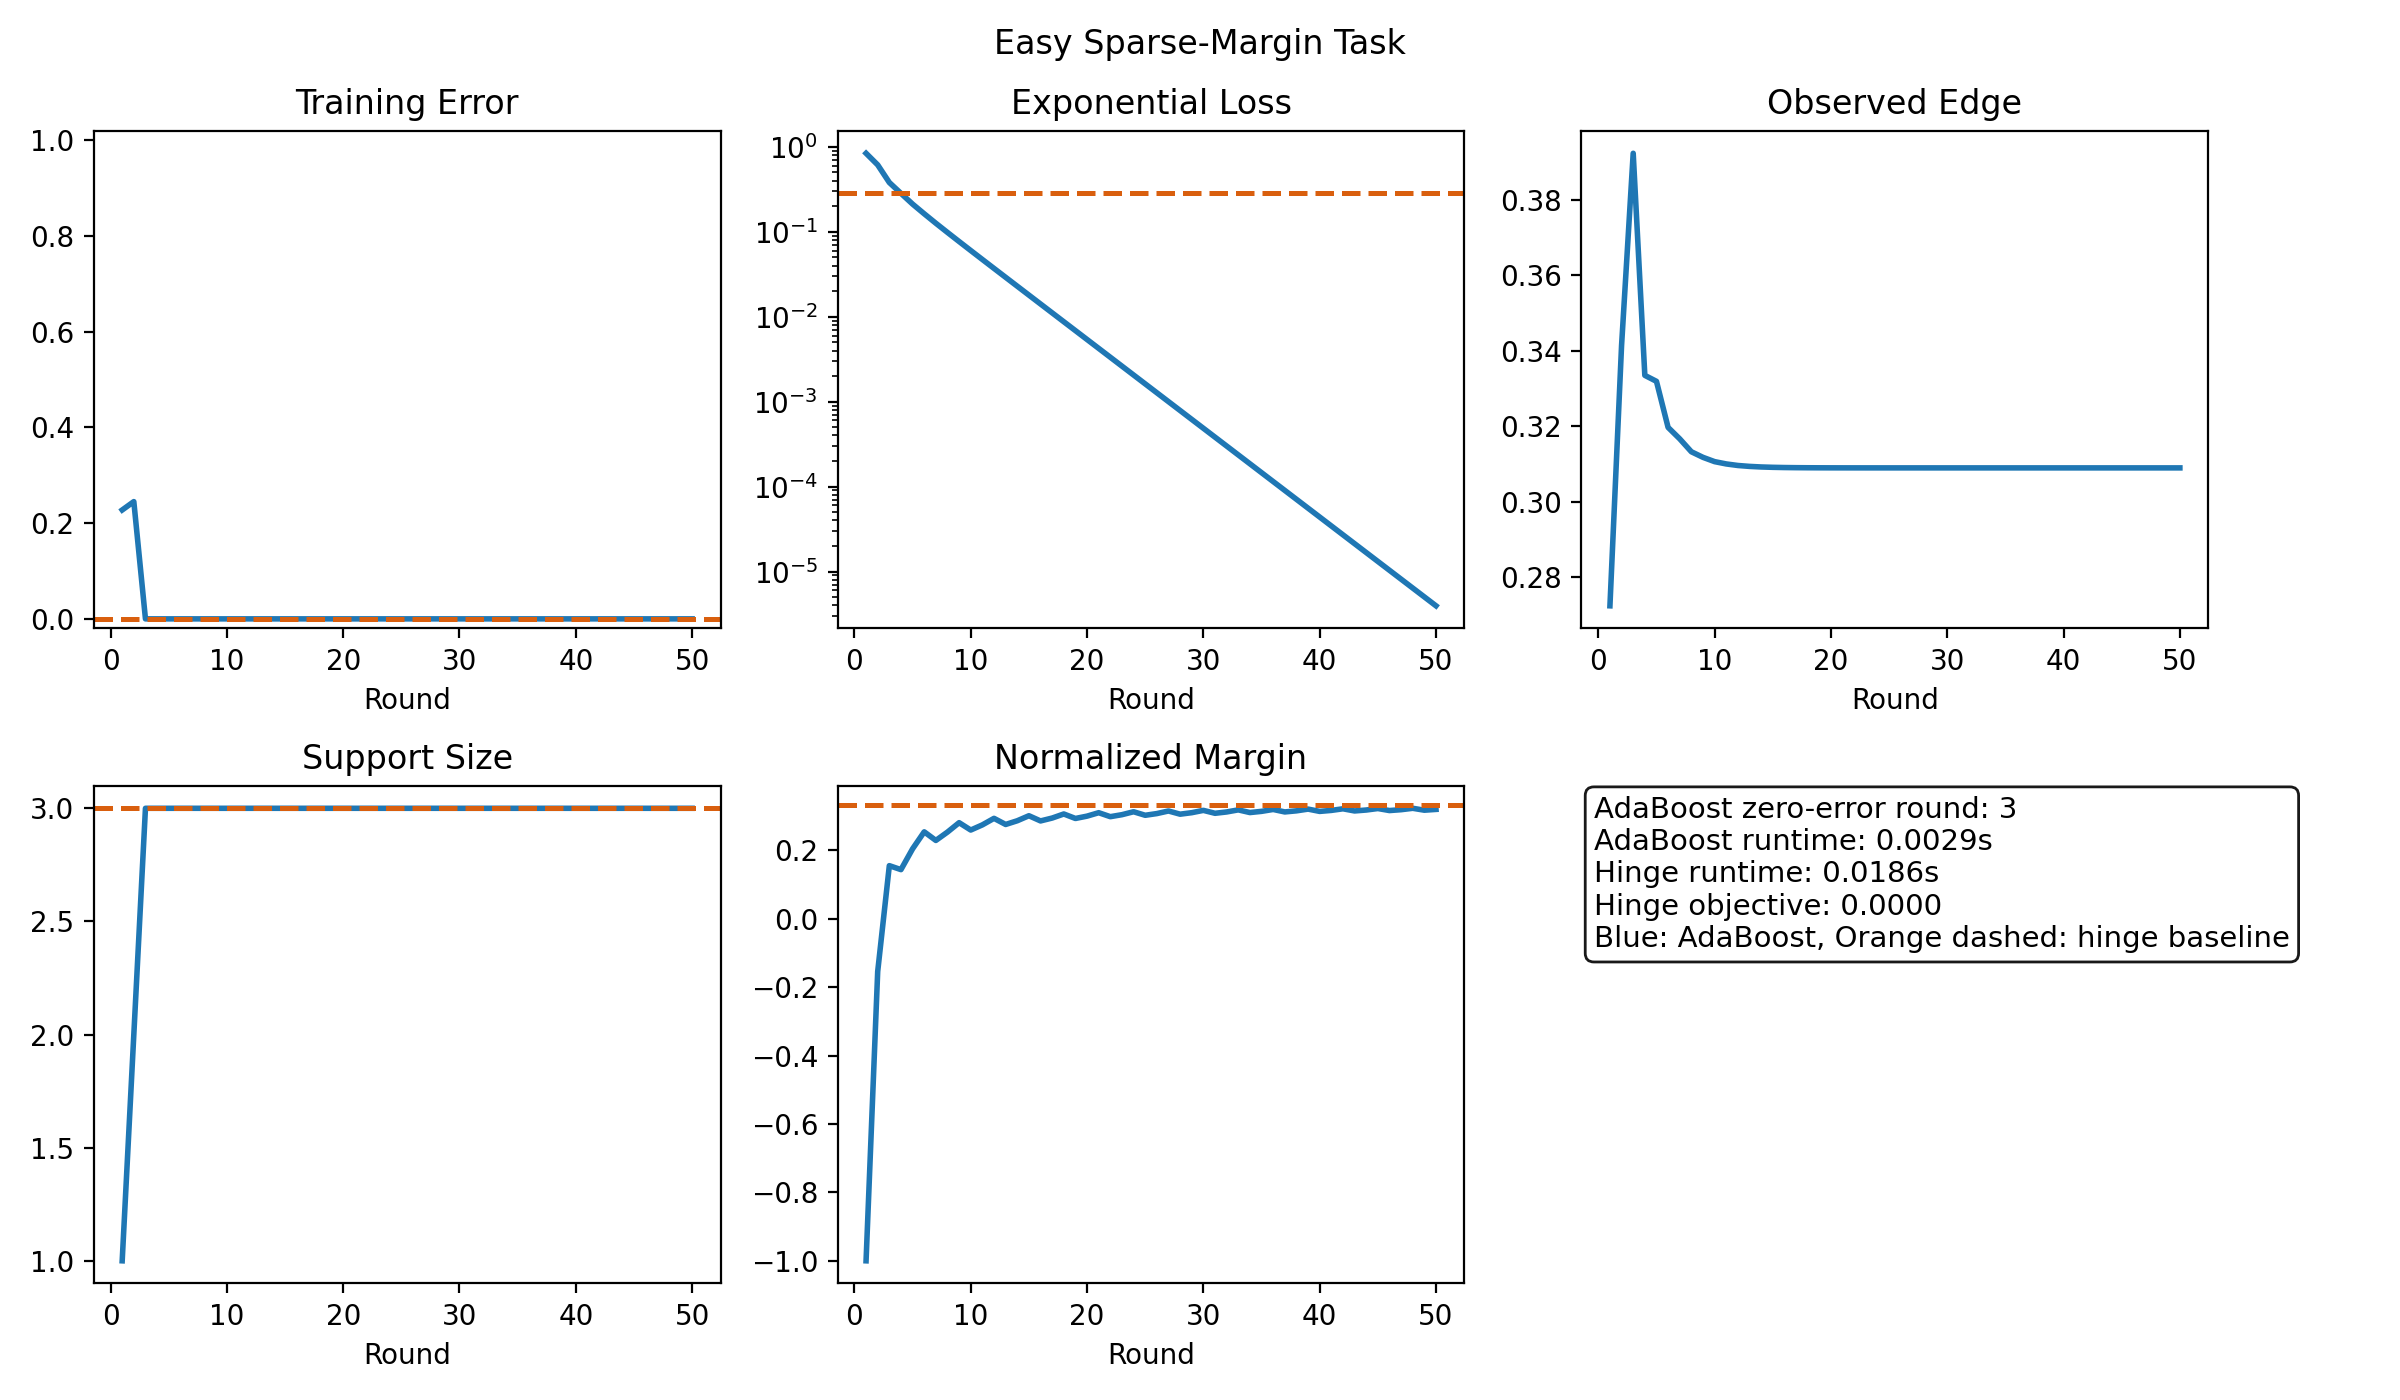
\includegraphics[width=1\linewidth]{figures/easy_round_metrics.png}
  \caption{AdaBoost versus hinge-$\ell_1$ on the easy sparse-margin task.}
  \label{fig:hw6-easy}
\end{figure}

\subsubsection{Hard Construction}

For the hard task, I used the construction from Problem 3 with
$$
m=3,
\qquad
s=7.
$$
The weighted distribution has
$$
q=(1,1,1,2,2,4,4),
$$
so the best coordinate edge is exactly
$$
\frac{1}{2(2^{m+1}-1)}=\frac{1}{30}\approx 0.0333,
$$
and the script observes an initial edge of $0.0333$ and a final edge of about $0.0318$ after $200$ rounds.

AdaBoost needed $136$ rounds before its training error became zero. Even after $200$ rounds, the normalized margin was only about
$$
0.0065,
$$
which is tiny compared with the easy task. The support size quickly saturated at $7$, so the real bottleneck was not support growth but the weak edge induced by poor $\ell_1$ geometry.

For the convex surrogate baseline, I used hinge-loss minimization with $\ell_1$ radius $7$. It did \emph{not} fit the sample: its training error stayed at $0.2$, its exponential loss was about $27.3$, and its normalized margin was negative. This is consistent with the theory: the hard instance has a margin-$1$ separator, but it requires large coefficients, and the witness from Problem 3 already has
$$
\|w^\star\|_\infty = 9.
$$

\begin{figure}[H]
  \centering
  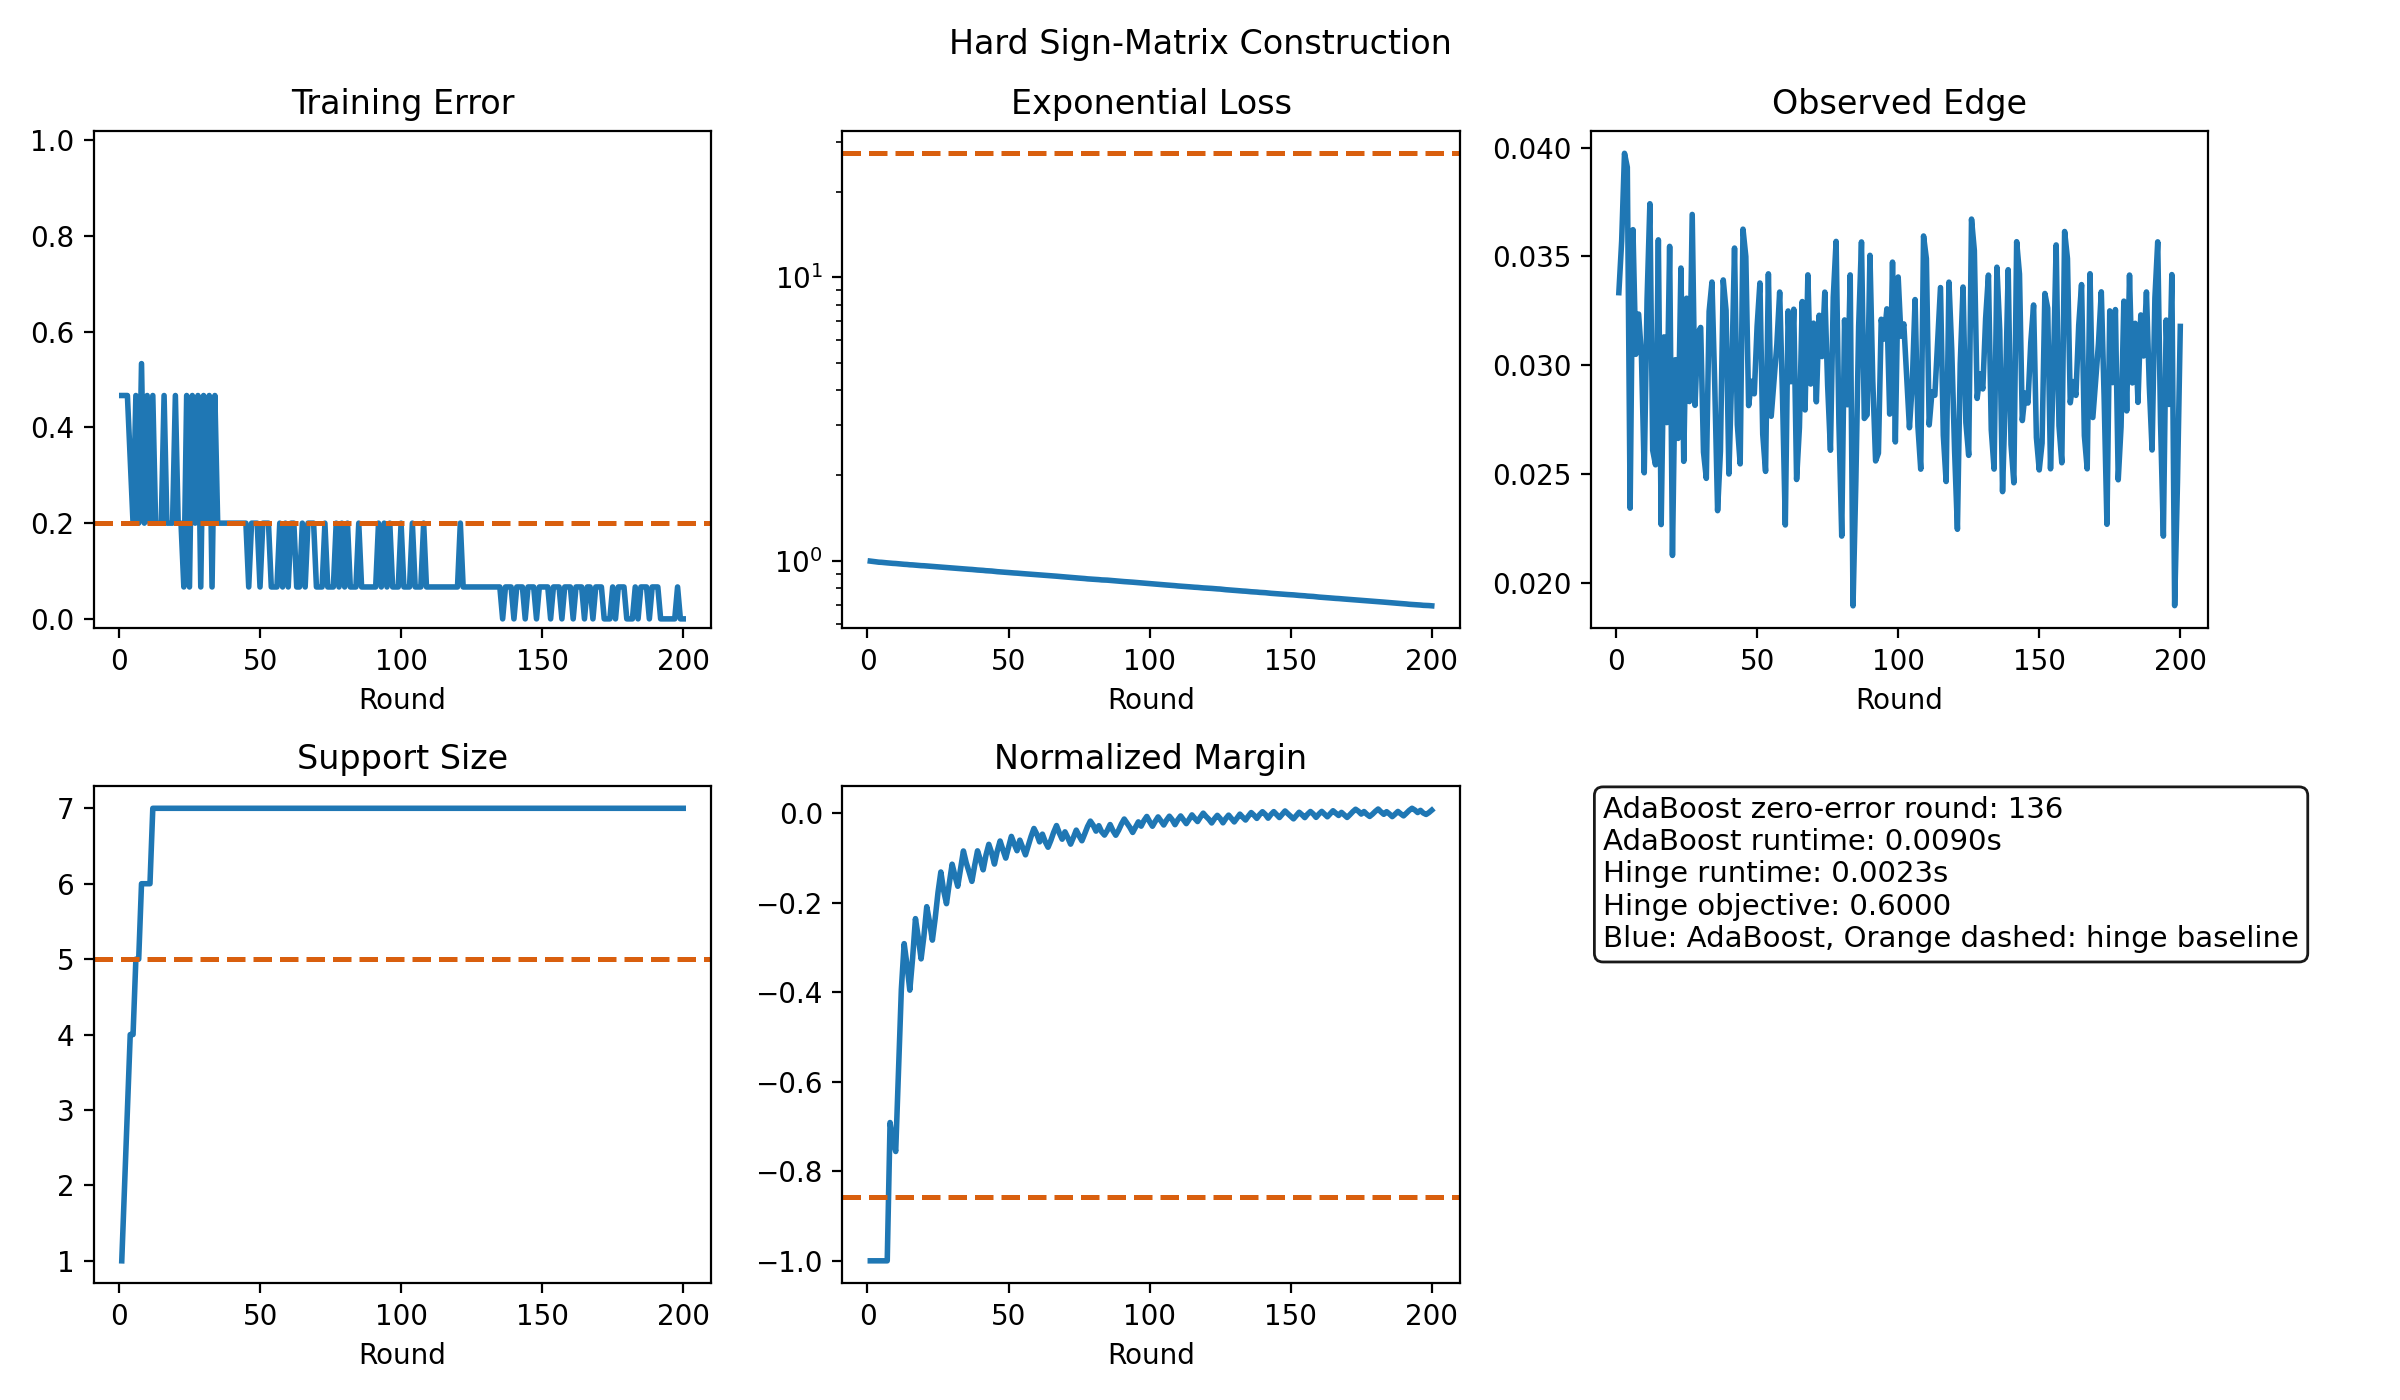
\includegraphics[width=1\linewidth]{figures/hard_round_metrics.png}
  \caption{AdaBoost versus hinge-$\ell_1$ on the hard sign-matrix construction.}
  \label{fig:hw6-hard}
\end{figure}

\subsubsection{Conclusion of the Experiment}

The experiment illustrates four points.
\begin{itemize}
\item Support sparsity alone is not enough. The easy and hard datasets are both sparse, but only the easy one gives a large coordinate edge.
\item Coefficient size matters because the weak-learning guarantee depends on $\|w^\star\|_1$, not just $\|w^\star\|_0$.
\item AdaBoost remains computationally cheap because each round is only a coordinate search, but it can need many rounds when the edge is tiny.
\item A convex surrogate with an $\ell_1$ constraint can work very well when the true separator has modest coefficient size, but it can fail badly when the margin witness requires large coefficients.
\end{itemize}

\newpage
\section{Part B: Agnostic Halfspace Hardness via Boosting}

\subsection{Problem 1. A Weak Halfspace Inside an Intersection}

Assume $\cD$ is realized by
$$
g(x)=\bigwedge_{r=1}^k h_r(x),
\qquad
h_r\in \cH_d.
$$
Let
$$
p := \PP_{\cD}[y=+1].
$$

\textbf{Case 1: $p \le \frac12-\frac{1}{2k}$.}
The constant classifier $h(x)\equiv -1$ is an affine halfspace, and its error is exactly $p$. Therefore
$$
L_{\cD}(h)=p \le \frac12-\frac{1}{2k} \le \frac12-\frac{1}{2k^2}.
$$

\textbf{Case 2: $p > \frac12-\frac{1}{2k}$.}
Whenever $y=+1$, realizability by the intersection implies
$$
h_r(x)=+1
\qquad
\text{for every }r\in[k].
$$
So each $h_r$ makes no error on positive examples.

Whenever $y=-1$, at least one of the $k$ halfspaces must output $-1$, otherwise the intersection would also output $+1$. Hence
$$
\frac{1}{k}\sum_{r=1}^k \PP_{\cD}[y=-1,\ h_r(x)=-1]
\ge
\frac{1-p}{k}.
$$
Therefore the average error of the $h_r$'s is
$$
\frac1k\sum_{r=1}^k L_{\cD}(h_r)
=
\frac1k\sum_{r=1}^k \PP_{\cD}[y=-1,\ h_r(x)=+1]
$$
$$
=
(1-p) - \frac1k\sum_{r=1}^k \PP_{\cD}[y=-1,\ h_r(x)=-1]
\le
(1-p)\left(1-\frac1k\right).
$$
Since in this case $p\ge \frac12-\frac{1}{2k}$,
$$
(1-p)\left(1-\frac1k\right)
\le
\left(\frac12+\frac{1}{2k}\right)\left(1-\frac1k\right)
=
\frac12-\frac{1}{2k^2}.
$$
So the average halfspace error is at most $\frac12-\frac{1}{2k^2}$, and therefore at least one affine halfspace satisfies
$$
L_{\cD}(h)
\le
\frac12-\frac{1}{2k^2}.
$$

\subsection{Problem 2. A Weak Learner from Proper Agnostic PAC Learning}

Assume, hypothetically, that affine halfspaces are efficiently \emph{properly} agnostically PAC learnable. I will use that learner as a subroutine on the weighted distributions generated by boosting.

Fix a distribution that is realizable by some intersection in $\cI_{d,k}$. By Problem 1, there exists an affine halfspace $h^\star$ with
$$
L(h^\star)\le \frac12-\frac{1}{2k^2}.
$$
Run the hypothetical proper agnostic learner with target excess accuracy
$$
\varepsilon_{\mathrm{agn}} := \frac{1}{4k^2}
$$
and constant confidence, say $2/3$. Since the learner is agnostic, it returns an affine halfspace $\widehat{h}$ such that
$$
L(\widehat{h})
\le
\inf_{h\in\cH_d} L(h) + \varepsilon_{\mathrm{agn}}
\le
\left(\frac12-\frac{1}{2k^2}\right)+\frac{1}{4k^2}
=
\frac12-\frac{1}{4k^2}.
$$
So this gives a weak learner with edge
$$
\gamma = \frac{1}{4k^2}.
$$

Why is it polynomial-time when $k(d)\le d^c$ for fixed $c$? Because then
$$
\frac{1}{\varepsilon_{\mathrm{agn}}}=4k(d)^2\le 4d^{2c},
$$
which is polynomial in $d$. Hence any runtime polynomial in $d$, sample size, and $1/\varepsilon_{\mathrm{agn}}$ remains polynomial.

\subsection{Problem 3. Boosting the Weak Learner}

Now run AdaBoost using the weak learner from Problem 2. At every round, the reweighted distribution is still supported on the same sample, and that sample is still realized by the same intersection in $\cI_{d,k}$. So every round has weak edge at least
$$
\gamma = \frac{1}{4k^2}.
$$

AdaBoost therefore satisfies the standard training-error bound
$$
\widehat{L}(H_T)
\le
\exp(-2\gamma^2 T)
=
\exp\!\left(-\frac{T}{8k^4}\right).
$$
Thus
$$
T=O(k^4\log n)
$$
rounds are enough to make the empirical training error zero on an $n$-point sample.

We are allowed to use the boosted-halfspace VC bound
$$
\VC(\text{boosted halfspaces with }T\text{ rounds})
=
\widetilde{O}(Td).
$$
Hence, once the boosted classifier is sample-consistent, the realizable VC theorem gives true error at most $\varepsilon$ with probability at least $1-\delta$ provided
$$
n
=
\widetilde{O}\!\left(
\frac{
Td+\log(1/\delta)
}{
\varepsilon
}
\right).
$$
Substituting $T=O(k^4\log n)$ yields, up to logarithmic factors,
$$
n
=
\widetilde{O}\!\left(
\frac{
dk^4+\log(1/\delta)
}{
\varepsilon
}
\right).
$$

For runtime, each of the $T$ rounds calls the proper agnostic halfspace learner once, so the total runtime is
$$
\widetilde{O}(k^4)\cdot \operatorname{poly}(n,d)
$$
when $k(d)\le d^c$. In particular, for polynomially bounded $k(d)$ this is still polynomial.

\subsection{Problem 4. The Hardness Contradiction}

Combine Problems 2 and 3. If affine halfspaces were efficiently properly agnostically PAC learnable, then for every polynomially bounded
$$
k(d)\le d^c
$$
we would obtain an efficient realizable learner for intersections of $k(d)$ affine halfspaces:
\begin{itemize}
\item Problem 2 converts the agnostic learner into a weak learner with edge $\gamma=\Theta(1/k(d)^2)$.
\item Problem 3 boosts that weak learner in polynomially many rounds and keeps the final sample and runtime bounds polynomial.
\end{itemize}
So intersections of polynomially many affine halfspaces would be efficiently learnable in the realizable case.

This contradicts the stated hardness facts.

Under the $\mathrm{uSVP}$ hardness assumption, take
$$
k(d)=d^r
$$
for any fixed $r>0$. The previous implication would give an efficient realizable learner for intersections of $d^r$ halfspaces, contradicting the black-box hardness statement.

Under $\mathrm{RSAT}$, take any polynomially bounded function with
$$
k(d)=\omega(1).
$$
Again the previous implication would yield an efficient realizable learner for that intersection class, contradicting the $\mathrm{RSAT}$ hardness statement.

Therefore the hypothetical premise must be false: efficient \emph{proper} agnostic PAC learning of affine halfspaces would contradict these hardness assumptions. In short, the boosting reduction shows that proper agnostic halfspace learning is at least as hard as realizable learning of intersections of many halfspaces.

\newpage
\section{Part C: AI Usage Report}

I used AI for three parts of this assignment: organizing the proof skeletons for Parts A and B, checking algebra in the hard construction from Part A.3, and drafting the experiment script for Part A.4.

The main suggestions I accepted were: reducing Problem A.1 to a correlation lower bound via $\|w^\star\|_1$, using the two-case argument with $p=\PP[y=+1]$ in Part B.1, and comparing the easy sparse-margin task with the explicit hard sign-matrix construction in the experiment.

I rejected or revised two kinds of suggestions. First, I did not leave Part A.3 as a vague existential construction; I replaced it with an explicit sign matrix and explicit coefficients. Second, I did not report the experiment only qualitatively; I verified the concrete quantities from the saved JSON output and inserted the actual observed values.

I verified the submission in two ways. For the theory parts, I checked each bound against the exact claim in the assignment and reworked the algebra where constants mattered. For the coding part, I ran \verb|code/boosting_experiment.py| inside the \verb|ai4lt| Conda environment, saved the figures and summary JSON, and then rebuilt the PDF with \verb|pdflatex|.

The five most recent workflow updates in this repo that mattered here were:
\begin{itemize}
\item using the shared \verb|ai4lt| Conda environment before homework work,
\item standardizing on \verb|pdflatex| for compilation,
\item keeping one companion statement file per homework folder,
\item storing code under the homework-local \verb|code/| directory and figures under \verb|figures/|,
\item referencing long code by relative path in the report instead of inlining it.
\end{itemize}

\end{document}
